% Template for Cogsci submission with R Markdown

% Stuff changed from original Markdown PLOS Template
\documentclass[10pt, letterpaper]{article}

\usepackage{cogsci}
\usepackage{pslatex}
\usepackage{float}
\usepackage{caption}

% amsmath package, useful for mathematical formulas
\usepackage{amsmath}

% amssymb package, useful for mathematical symbols
\usepackage{amssymb}

% hyperref package, useful for hyperlinks
\usepackage{hyperref}

% graphicx package, useful for including eps and pdf graphics
% include graphics with the command \includegraphics
\usepackage{graphicx}

% Sweave(-like)
\usepackage{fancyvrb}
\DefineVerbatimEnvironment{Sinput}{Verbatim}{fontshape=sl}
\DefineVerbatimEnvironment{Soutput}{Verbatim}{}
\DefineVerbatimEnvironment{Scode}{Verbatim}{fontshape=sl}
\newenvironment{Schunk}{}{}
\DefineVerbatimEnvironment{Code}{Verbatim}{}
\DefineVerbatimEnvironment{CodeInput}{Verbatim}{fontshape=sl}
\DefineVerbatimEnvironment{CodeOutput}{Verbatim}{}
\newenvironment{CodeChunk}{}{}

% cite package, to clean up citations in the main text. Do not remove.
\usepackage{apacite}

% KM added 1/4/18 to allow control of blind submission


\usepackage{color}

% Use doublespacing - comment out for single spacing
%\usepackage{setspace}
%\doublespacing


% % Text layout
% \topmargin 0.0cm
% \oddsidemargin 0.5cm
% \evensidemargin 0.5cm
% \textwidth 16cm
% \textheight 21cm

\title{Analyzing contingent interactions in R with \texttt{chattr}}


\author{{\large \bf Marisa Casillas (mcasillas@uchicago.edu)} \\ Comparative Human Development, 1101 E. 58th St. \\ Chicago, IL 60637 USA \AND {\large \bf Camila Scaff (camila.scaff@iem.uzh.ch)} \\ Institute of Evolutionary Medicine, University of Zurich \\ Zurich, Switzerland CH-8057}


\begin{document}

\maketitle

\begin{abstract}
We present \texttt{chattr}, an R package that enables users to easily
detect and describe temporal contingencies in pre-annotated
interactional data. The need to detect and analyze temporal
contingencies is ubiquitous across studies of signal exchange systems,
including human and non-human animal communication systems. At present,
approaches to this kind of analysis require careful manual evaluation
(i.e., do not scale up), are proprietary and/or over-specialized (i.e.,
are limited in use), or are constructed ad-hoc for each study (i.e., are
variable in construct). \texttt{Chattr}`s theoretically motivated,
customizable, and open source code provides a set of core functions that
allow users to quickly and automatically extract contingencies in data
that have already been annotated for interactant activity (via manual or
automated application) in one of multiple common data formats (.txt,
.rttms, .its). Particularly given the rise of powerful, long-lasting
recording devices and automated tools for diarizing activity in these
recordings, \texttt{chattr} stands to facilitate valid at-scale analysis
of temporal contingencies in a wide variety of data types while also
providing consistency across studies in the analytical approach.
Detailed output includes information about related turns ('prompts' and
`responses') and the allocation of turns into interactional sequences
(`conversational bouts') and solo sequences (`monologues') for every
emission produced by a target interactant. We here demonstrate the use
of \texttt{chattr} by testing predictions about turn-taking behavior in
three language development corpora, showing that the package effectively
recovers documented variation in linguistic input given both manual and
automatically created speech annotations. We note future directions for
package development, with the hope that it will be used for the
convenient management and analysis of interactional data across multiple
distinct research contexts.

\textbf{Keywords:}
Contingency; interaction; turn taking; LENA; communication;
conversation; R; automated speech annotation.
\end{abstract}

\hypertarget{introduction}{%
\section{Introduction}\label{introduction}}

The current paper introduces an R (REFS) package called \texttt{chattr}
that facilitates the detection and analysis of temporally contingent
interactions in pre-annotated data (URL redacted).\footnote{At time of
  submission, the conversion from R scripts to R package is still
  underway. That said, all documentation, scripts, and tests are
  available at the given URL and the fully packaged version will be
  available before May 2021.} The utility of this package extends across
studies of adult and child human interactions, non-human animal
communication, and contingencies within multi-modal signals. Despite
significant common conceptual ground between these domains, definitions
of contingency phenomena and implementations of contingency detection
remain fairly inconsistent, foregoing critical opportunities for the
accumulation of shared construct validity across domains. In part, these
divergences are due to the lack of flexible tools for contingency
analysis; existing systems are either constructed ad-hoc or are
proprietary, and thereby limited in who can use them. The
\texttt{chattr} package aims to improve this situation in two ways: (1)
It takes inspiration from the fields of conversation analysis,
psycholinguistics, and language development to provide theoretically
sound, but customizable measurements of temporally contingent
interaction at scale and (2) its open-source toolkit accepts a handful
of generic formats as input, opening up its analytical framework to a
wide variety of domains (e.g., child language input, multi-party adult
conversation, non-human animal signal exchanges, multi-modal
contingencies produced by a single organism, etc.). The remainder of
this short report reviews the theoretical basis underlying the
development of \texttt{chattr}, describes the core functions offered by
the package, and demonstrates its use in three existing datasets.

\begin{CodeChunk}
\begin{figure*}[h]

{\centering 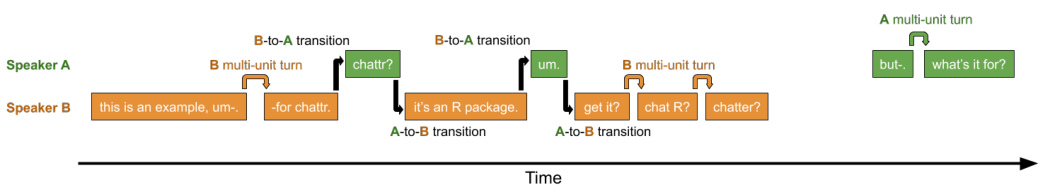
\includegraphics{figs/minisequence-1} 

}

\caption[An example of a brief dyadic interaction between two English speakers]{An example of a brief dyadic interaction between two English speakers: A (green) and B (orange). The producers here use both single- and multi-unit turns. There are 6 turns (3 from each producer), 4 turn transitions (two each from B to A and vice versa; black arrows), and one interactional sequence (the contiguous block of producer continuation/transition marked with green/orange arrows; the other turn ('but-. what's it for?') has no transitions and so is not an interactional sequence).}\label{fig:minisequence}
\end{figure*}
\end{CodeChunk}

\hypertarget{contingent-interaction}{%
\subsection{Contingent interaction}\label{contingent-interaction}}

The joint coordination of action by two or more agents usually involves
temporal contingencies. Whether we are making music with others,
crossing a busy intersection, or chatting with a friend, the timing of
our contributions to a coordinated event is crucial to its success. In
many cases, the optimal strategy for coordination involves some form of
turn taking. In a typical turn-taking interaction, only one interactant
makes their contribution at a time, and decisions about who contributes
when can be determined flexibly (as in conversation) or in a pre-defined
manner (as in a debate). This sequential structure enables interactants
to adapt each contribution such that it relevantly progresses the joint
activity and to initiate unplanned subsequences (e.g., repairing a
misunderstanding) without breaking from moving toward the the larger
goal.

Turn-taking (and similar temporally contingent) interactions are
essential for communication across the animal kingdom (REFS). In humans,
turn-taking interactions may be the only reliable source of language
universals (REFS). Traditionally, these kinds of interactional
contingencies have been studied using careful inspection and analysis
(both qualitative and quantitative) of manual measurements from video
and audio recordings. However, recent advances in automated annotation
tools (e.g., tools for voice detection) have opened up the possibility
to investigate interactional behavior at a much larger scale, creating a
need for new, and validated analytical approaches.

\hypertarget{current-contingency-detection-approaches-and-their-limitations}{%
\subsection{Current contingency detection approaches (and their
limitations)}\label{current-contingency-detection-approaches-and-their-limitations}}

At present, the most widely used tool with respect to automated
contingency analysis of human interaction is the LENA system (REFS). The
LENA system was built to be used with young children, but has also been
employed to capture adult language environments (REFS). The system
includes both a recording device and a set of proprietary software tools
that enable the user to first collect long-format (16-hour)
participant-centric audio recordings and second, automatically analyze
them for a range of properties, such as when vocalizations occur by
speakers of different types (e.g., near/far female adult vocalizations).
The software then uses the detected vocalizations to find candidate
regions of vocal exchange (VABs; Vocal Activity Blocks) between the
target child and nearby adults. It then calculates the estimated number
of speaker exchanges that involve the child, using temporal contingency
to associate speaking turns from different speaker types (i.e.,
\textless5 seconds of silence between child and woman/man vocalizations
or vice versa). This extremely convenient system, which has been
critical to spurring on new research on language development and
turn-taking (REFS) has a few unfortunate drawbacks. Reliability
estimates for turn count estimates are between 0.3 and 0.6 (REFS;
Bulgarelli et al., under review; Cristia et al., under review), with
systematically worse errors for younger infants than older ones
(REFS).\footnote{Note that most CTC error estimates inherit error from
  earlier steps in the processing pipeline (e.g., misidentifying speech
  as silence).} The system is also proprietary, expensive, and can only
be used with recordings made with the LENA hardware. Therefore, research
groups who lack generous funding or who have unique hardware and storage
requirements will struggle to benefit from the system. Lastly, LENA is
designed specifically for child-centric recordings, improving the
accuracy of its application in the developmental language context, but
offering minimal utility for those working in other domains.

\begin{CodeChunk}
\begin{figure*}[h]

{\centering 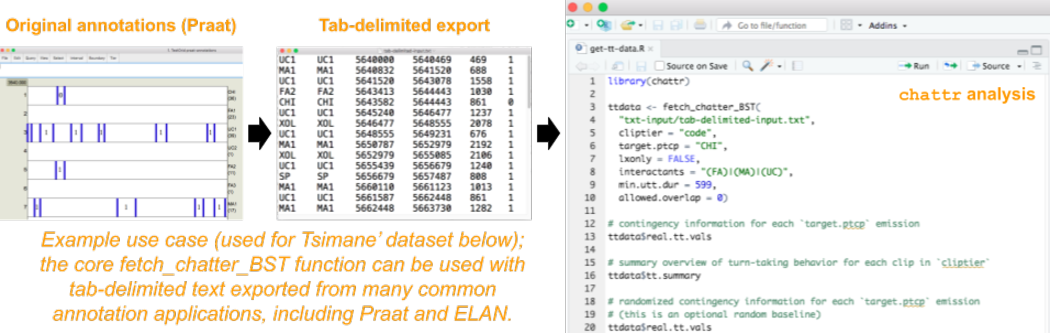
\includegraphics{figs/workflow-1} 

}

\caption[Example workflow for an annotation file using `chattr`]{Example workflow for an annotation file using `chattr`.}\label{fig:workflow}
\end{figure*}
\end{CodeChunk}

Beyond LENA, approaches to extracting temporal contingencies over whole
corpora have been much more variable. For example, in studies of adult
conversation, researchers vary in what timing windows qualify as
contingent, what types of contributions count toward turn taking, the
modality in which communication is taking place, in how many
interactants are considered to be involved (or are of interest), and so
on, as is suitable to the research question (REFS; Roberts et al (2015)
Heldner \& Edlund? Bosch Animal studies??). These studies, while
heterogenous in data types and determinants for how and when to count
turn-taking exchanges, have typically been inspired by core concepts
from conversation analysis, building up significant theoretical common
ground for understanding moment-to-moment processes of interactant
coordination. Much of the work on language development, by contrast, has
inherited the somewhat idiosyncratic concepts and terminology introduced
by the LENA system, leaving a conceptual disjunct between work on
turn-taking behaviors in children, adults, and non-human animals. Given
the various restrictions on existing tools and free variations in
analysis across studies, there is a clear need for a free, flexible, and
theoretically grounded tool that can extract temporal contingencies at
scale; \texttt{chattr} aims to fill this need. The following text
briefly describes the package and its use before turning to examples
with real datasets from the child language literature.

\hypertarget{the-chattr-system}{%
\section{\texorpdfstring{The \texttt{chattr}
system}{The chattr system}}\label{the-chattr-system}}

In brief, \texttt{chattr} is an R package that gives both summary and
detailed data on temporal contingencies in pre-annotated data. To keep
things simple, it has a single core function for each type of input that
it takes: (a) LENA .its files; (b) tab delimited .txt tables with one
production (i.e., utterance) per row, as can be exported from Praat,
ELAN, and so forth (REFS); and (c) .rttm tables, a common output format
used with automated speech diarization systems.\footnote{Users
  interested in a fully open-source pipeline for child language
  environments should check out Lavechin et al.'s (REFS) voice type
  classifier.}

Users can use the default settings for each function---which include
limits on the relevant temporal windows, potential interactants, and
restrictions on productions considered---or can customize as desired.
More advanced users can capitalize on the wide variety of sub-functions
utilized by the core input-type functions to tailor \texttt{chattr}'s
functions to their unique needs. All settings, output information types,
and theoretical background is thoroughly summarized in the online
documentation where the project is stored on GitHub.

\hypertarget{core-concepts}{%
\subsubsection{Core concepts}\label{core-concepts}}

We encourage users to first evaluate how well \texttt{chattr}`s concepts
of 'turn', `transition', and `interactional sequence' fit those of the
user; our default definitions differ from those typically used in the
language development literature and are somewhat restricted compared to
their full (and human conversation-specific) theoretical meanings in
conversation analysis (e.g., see REFS). We briefly summarize these core
concepts here. The same concepts are illustrated in Figure 1. We use the
concepts of `producer' and `recipient'/`addressee' rather than `speaker'
and `listener' to underscore the utility of these concepts across
modalities, species, and interactional contexts:

A \emph{`turn'} comprises one or more closely occurring emissions by the
same producer. That is, a turn can be formed of multiple complete
emissions (e.g., utterances/communicative acts) that may be separated by
pauses in production so long as (a) there is no intervening emission
from another producer and (b) the pause in production is short. An
example of a single-unit turn in English is ``Jane is the one in the
hat.''. An example of a multi-unit turn in English is ``Jane is the one
in the hat {[}pause{]} third from the left.''.

A \emph{`turn transition'} occurs when one producer's turn stops and
another producer's turn begins. Every turn transition has a
pre-transition producer and a post-transition producer---these must be
different individuals. The transition \emph{begins} when the first turn
ends and \emph{ends} when the second turn starts. Therefore, if the
second turn starts before the first turn ends, the transition time is
negative; this is referred to as `transitional overlap'. If the second
turn starts after the first turn ends, the transition time is positive;
referred to as `transitional gap'.

An \emph{`interactional sequence'} is an unbroken turn-taking sequence
between the target interactant and one or more of their interactional
partners. Interactional sequences likely index more structurally
complex, engaged interactional behaviors than single turn transitions
do---akin to conversational bouts (or LENA VABs)---in which participants
can more substantially build on joint goals.

Default settings are designed for human spontaneous conversation,
including conversation, which demonstrates fairly robust timing patterns
(with some systematic variation) across the signed and spoken languages
that have been analyzed (REFS). The three most critical default settings
are that: (a) up to 2000 ms of transitional gap or up to 1000 ms of
transitional overlap is allowed between turns, (b) turn transitions can
occur with turns of any duration, content, and between any potential
interactional partner, and (c) when there are multiple potential prompts
or responses (e.g., two interactants answer a question nearly
simultaneously), \texttt{chattr} picks the turn that begins soonest.
Users interested in emulating LENA's CTC measure with their .its files
can use a specialized version of the tool in which the target producer
is assumed to be ``CH'' (target child), potential interactants limited
to ``FA'' and ``MA'' (female and male adult), and analyzed turns contain
some linguistic material (REFS).

\hypertarget{example-use-case}{%
\subsubsection{Example use case}\label{example-use-case}}

Suppose that I am interested in investigating how adult turn-taking
varies in a dataset across semi-structured contexts (e.g., during board
game play). I would ensure that the annotations are formatted as
tab-delimited text (see the \texttt{chattr} documentation). Then I would
use the Basic Speech Table call \texttt{fetch\_chatter\_BST()} to fetch
turn-taking information. I might also desire to, e.g., employ a minimum
utterance duration and a more strict temporal window for contingency, as
well as calculate 10 randomized simulations of turn-taking rates to
assess the baseline likelihood of finding a contingency:
\texttt{fetch\_chatter\_BST(filename,\ min.utt.dur\ =\ 1500,\ allowed.gap\ =\ 1000,\ allowed.overlap\ =\ 600,\ n.runs\ =\ 10)}.
This call yields detailed tables of detected turn-taking behavior ready
for the author's statistical analysis of choice (Figure 2).

\hypertarget{pilot-analysis}{%
\section{Pilot analysis}\label{pilot-analysis}}

We demonstrate the use of \texttt{chattr} with three child language
environment datasets from rural Indigenous communities. These recordings
document children's verbal interactional patterns over full waking days
at home in underrepresented research populations. \texttt{Chattr} allows
us to examine interactional patterns at scale in these corpora, evading
months of manual annotation achieving the same aim. The first two
corpora, Tseltal (Mayan; Chiapas, Mexico; N = 10) and Yélî Dnye
(isolate; Milne Bay, Papua New Guinea; N = 10), come from the Casillas
HomeBank corpus (REFS) and were made with near parallel methods:
children under age 3;0 wore an Olympus WS-832/853 audio recorder during
a day at home for 8--11 hours. The third corpus, Tsimane' (Tsimane';
Bolivia; N = 27) features children under 6;0 who wore one of multiple
recording devices (LENA, Olympus, or USB) during a day at home for 4--21
hours (REFS); we focus here on the subset of those 27 recordings made
with LENA (N = 17). In each dataset we assess the baseline turn-taking
rate and duration of interactional sequences over age and by interactant
type. For the Tsimane' corpus we briefly compare \texttt{chattr}
estimates on both LENA (automated) and manually created annotations of
the same recording minutes. Here \texttt{chattr} gives a brief glimpse
into how reliably known patterns from these children's linguistic input
(REFS) are recapitulated in their turn-taking behavior.

\hypertarget{study-1.-tseltal-and-yuxe9luxee-dnye}{%
\subsection{Study 1. Tseltal and Yélî
Dnye}\label{study-1.-tseltal-and-yuxe9luxee-dnye}}

We analyze interactional behavior in 20 clips for each recording: 9
randomly selected clips (5 min for Tseltal and 2.5 min for Yélî Dnye), 5
clips manually selected for day-peak turn-taking behavior of the target
child with one or more interactants (each 1 min), 5 clips manually
selected for day-peak vocal activity by the target child (each 1 min),
and one 5-minute expansion on the most active turn-taking or vocal
activity clip. Each clip was manually annotated for all hearable speech,
including addressee coding (e.g., target-child-directed
vs.~other-directed; see REFS for details). Despite documented
differences in caregiver-child interactional style (REFS), day-long
linguistic input estimates show similar directed linguistic input
patterns in these two communities. While female adult speech constitutes
the majority of linguistic input in both communities, Yélî children show
a marked increase in directed speech from other children with age. This
pattern appears more weakly in the Tseltal data. We therefore expected
to find that: (1) turn-taking rates are higher in turn-taking clips than
in vocal activity and random clips, (2) rates are overall similar
between the two communities, and (3) interactional sequences involving
other children increase with age, particularly for Yélî children.

\begin{CodeChunk}
\begin{figure}[h]

{\centering 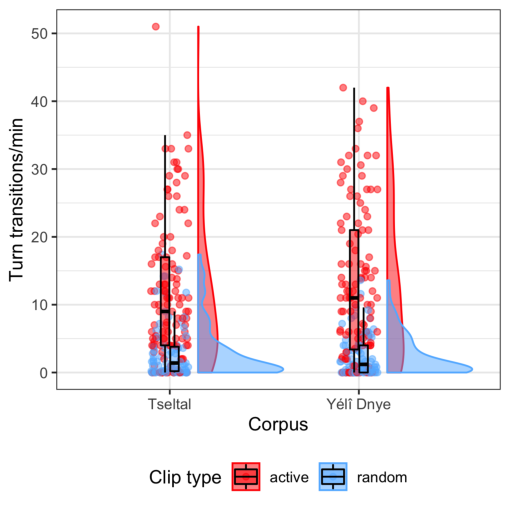
\includegraphics{figs/tseyel.ttr.fig-1} 

}

\caption[Turn transition rate by corpus, divided across random (blue) and manually selected turn-taking/high-vocal-activity clips (red)]{Turn transition rate by corpus, divided across random (blue) and manually selected turn-taking/high-vocal-activity clips (red).}\label{fig:tseyel.ttr.fig}
\end{figure}
\end{CodeChunk}

\begin{CodeChunk}
\begin{figure}[h!]

{\centering 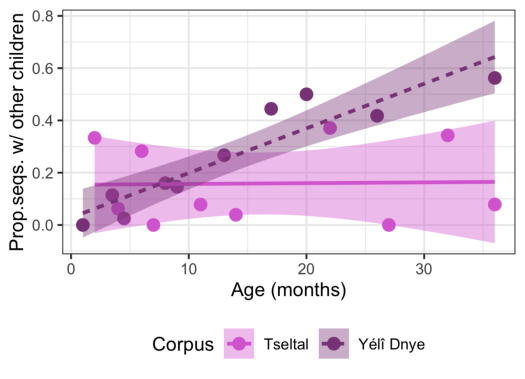
\includegraphics{figs/tseyel.is.fig-1} 

}

\caption[Proportion of interactional sequences involving at least one non-target child across age, by language]{Proportion of interactional sequences involving at least one non-target child across age, by language.}\label{fig:tseyel.is.fig}
\end{figure}
\end{CodeChunk}

\hypertarget{methods}{%
\subsubsection{Methods}\label{methods}}

We use the \texttt{fetch\_chatter\_AAS()} call, which is specifically
designed for those using the ACLEW Annotation Scheme (REFS){[}\^{}4{]}:
that allows 2000 ms of gap and 1000 ms of overlap between at turn
transitions and searches over all annotated utterances (any duration,
content, and from any speaker). We limit our analysis to utterances
directed exclusively to the target child. We also indicate the annotated
regions by using the \texttt{cliptier} argument (see documentation).

{[}\^{}4{]} ACLEW is a working group that has provided a flexible manual
annotation template friendly for use with open source speech processing
tools (REFS).

\hypertarget{results}{%
\subsubsection{Results}\label{results}}

The mean rate of turn transitions in the Tseltal corpus was 3 and 11.8
transitions per minute for the random and active clips, respectfully.
The mean rates in the Yélî Dnye corpus were 2.4 and 12.8 for the random
and active clips. Overall the distribution of turn taking rates across
annotated clips was similar between the two sites (Table 1). A linear
mixed effects regression of turn-transitions per minute with predictors
of clip type, corpus, and their interaction and a random intercept for
child reveals that, indeed, random clips have significantly lower
turn-transition rates (B = -8.78, SE = 1.2, t = -7.31) and there is no
evidence for a significant difference in turn-taking rates between
languages (t = 0.54) and no evidence for a clip type-language
interaction (t = -0.74).

A second linear mixed effects regression of the proportion of
interactional sequences that feature at least one non-target child with
predictors of age (in months), corpus, and their interaction and a
random intercept for child reveals that, as expected, there is a
significant age-by-corpus interaction by which Yélî children show a
larger increase in other-child interactional sequences with age compared
to Tseltal children (B = 0.01, SE = 0.01, t = 2.47). There is no
evidence for simple effects of age (t = 0.2) or language (t = -0.99).

\hypertarget{study-2.-tsimane}{%
\subsection{Study 2. Tsimane'}\label{study-2.-tsimane}}

These Tsimane' recordings were first automatically analyzed with LENA
and then subsequently (and independently) manually annotated in one
minute clips, every 60 minutes, starting at the 34th minute (34 min, 94
min, 154 min, etc.) in Praat (REFS). Both annotation formats include
information regarding (a) when speech was occurring and (b) what type of
speaker produced it (i.e., the target child, a nearby woman/man/other
child, or other noise sources) for each of the hand-annotated minutes.
Prior analysis shows comparably low rates of directed speech in these
Tsimane' data to the Tseltal and Yélî Dnye recordings, again with a high
proportion of directed input coming from other children. We therefore
expected to find that: (1) turn-taking rates are overall similar to what
we found in the random samples of the other two communities, (2)
turn-taking sequences involving other children are comparable or more
frequent than found in the random samples of the other two communities,
(3) interactional sequences involving other children increase with age,
and (4) manual and automated speech annotations of the same audio clips
result in similar turn-taking estimates.

\begin{table}[h]
\centering
\begin{tabular}{lll}
  \hline
Corpus & Clip type & mean (sd; range), median \\ 
  \hline
Tseltal & active (manual) & 11.8 (4.8; 4.5-20.1), 12.3 \\ 
  Tseltal & random (manual) & 3 (3.1; 0.4-10.6), 2.3 \\ 
  Yélî Dnye & active (manual) & 12.8 (6.5; 3.9-22.2), 10.8 \\ 
  Yélî Dnye & random (manual) & 2.4 (1.6; 0.5-6), 2.2 \\ 
  Tsimane' & random (LENA) & 3.2 (1.1; 1.2-5.1), 3.1 \\ 
  Tsimane' & random (manual) & 3.2 (1.2; 1.3-6), 3 \\ 
   \hline
\end{tabular}
\end{table}

\begin{CodeChunk}
\begin{figure}[h]

{\centering 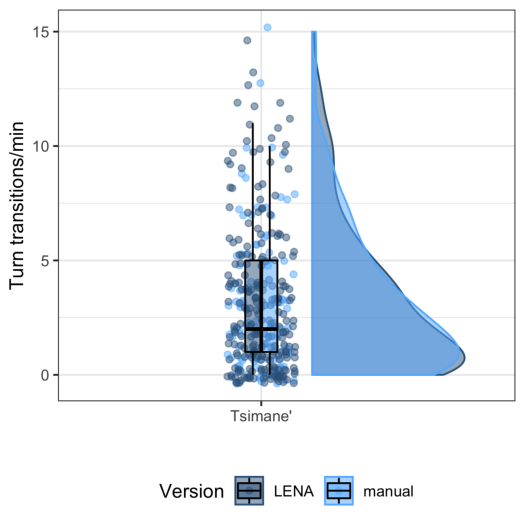
\includegraphics{figs/tsi.ttr.fig-1} 

}

\caption[Turn transition rate by annotation type (LENA automated vs]{Turn transition rate by annotation type (LENA automated vs. manual) in the same audio clips. Clips are a periodic random sample of the daylong recording.}\label{fig:tsi.ttr.fig}
\end{figure}
\end{CodeChunk}

\begin{CodeChunk}
\begin{figure}[h!]

{\centering 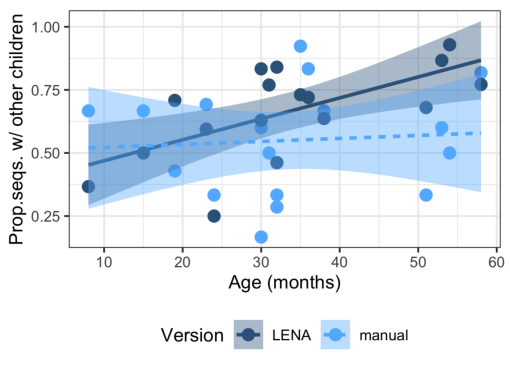
\includegraphics{figs/tsi.is.fig-1} 

}

\caption[Proportion of interactional sequences involving at least one non-target child across age, by annotation type (LENA automated vs]{Proportion of interactional sequences involving at least one non-target child across age, by annotation type (LENA automated vs. manual) in the same audio clips.}\label{fig:tsi.is.fig}
\end{figure}
\end{CodeChunk}

\hypertarget{methods-1}{%
\subsubsection{Methods}\label{methods-1}}

We first use the \texttt{fetch\_chatter\_BST()} call with the manually
annotated data, matching conditions of the call as closely as possible
to what can be compared in the LENA output files, that is: include
woman, man, and other-child speech, both linguistic and non-linguistic,
with a minimum utterance duration of 600ms (the LENA lower limit) and no
overlap allowed (meaningful overlap is not possible in LENA). With the
automatic LENA annotations on the same recordings (in the same 1-minute
segments) we adjust the defaults on \texttt{fetch\_chatter\_LENA()} to
reflect the same restrictions.

\hypertarget{results-1}{%
\subsubsection{Results}\label{results-1}}

A linear mixed effects regression of turn-transitions per minute with
predictors of annotation type (LENA automated vs.~manual) and a random
intercept for child reveals that turn-transition rates are similar
between the two annotation methods (B = -0.09, SE = 0.41, t = -0.23).
Consistent with our hypothesis, the mean rate of turn transitions was
similar to what we found in the Tseltal and Yélî Dnye random clips, at
3.2 transitions per minute, though with fewer instances of rates above
5/min (Table 1).

A second linear mixed effects regression of the proportion of
interactional sequences that feature at least one non-target child with
predictors of age (in months), annotation type (LENA vs.~manual), and
their interaction and a random intercept for child reveals that, as
expected, there is a significant increase in other-child interactional
sequences with age (B = 0.01, SE = 0, t = 3.39). There is no evidence
for simple effects of annotation type (t = 0.71) or for an
age-annotation type interaction (t = -1.39).

\hypertarget{contribution-and-next-steps}{%
\section{Contribution and next
steps}\label{contribution-and-next-steps}}

The \texttt{chattr} package allows users to easily implement
theoretically informed contingency analyses on a wide variety of data
types, including both automatically and manually annotated data. The
package is designed for both straightforward (i.e., basic
\texttt{fetch\_chatter} calls) and customized analysis scenarios and
provides detailed outputs that can be merged with other data about the
same recordings. By providing a single tool for analyzing the most
common input formats used for interactional data in psychology, animal
behavior, and speech technology research, \texttt{chattr} aims to help
build theoretical and methodological connections regarding the nature of
contingent behaviors across diverse domains. While \texttt{chattr} has
now been tested on a variety of child language datasets, new
functionality will emerge following issue posting and feature requests
by users. Following this beta stage of development we will make the
package available on CRAN for easier distribution. A critical next step
will also be the development of tutorial materials to accompany the
documentation, enabling new R users to quickly apply the core functions
to a sampling of common use cases.

\hypertarget{acknowledgements}{%
\section{Acknowledgements}\label{acknowledgements}}

REDACTED

\hypertarget{references}{%
\section{References}\label{references}}

\setlength{\parindent}{-0.1in} 
\setlength{\leftskip}{0.125in}

\noindent

\bibliographystyle{apacite}


\end{document}
